% Kelompok 3
% Ajrina Dharman (1154079)
% Diana Satima G (1154018)
% Indah Rahmawati (1154070)
% M. Amran Hakim Siregar (1154106)
% Rizky Abdul Ghani Suherli (1154048)

\section{Peta}
	peta itu menggambaran  grafis atau bentuk skala (perbandingan) didalam konsep mengenai bumi. Pada bagian ini peta merupakan alat untuk menyampaikan atau menginformasikan mengenai ilmu kebumian. Di dalam peta dahulu ditemukan ? pengetahuan mengenai dasar pembentukan peta sama seperti filosofi, yang mana sering terdapat perbedaan.

\subsection{Peta Menurut Abu Abdullah Muhammad al-Idrisi al-Qurtubi al-Hasani as-Sabti "al-Idrisi"}
	\begin{figure} [ht]
	\centerline{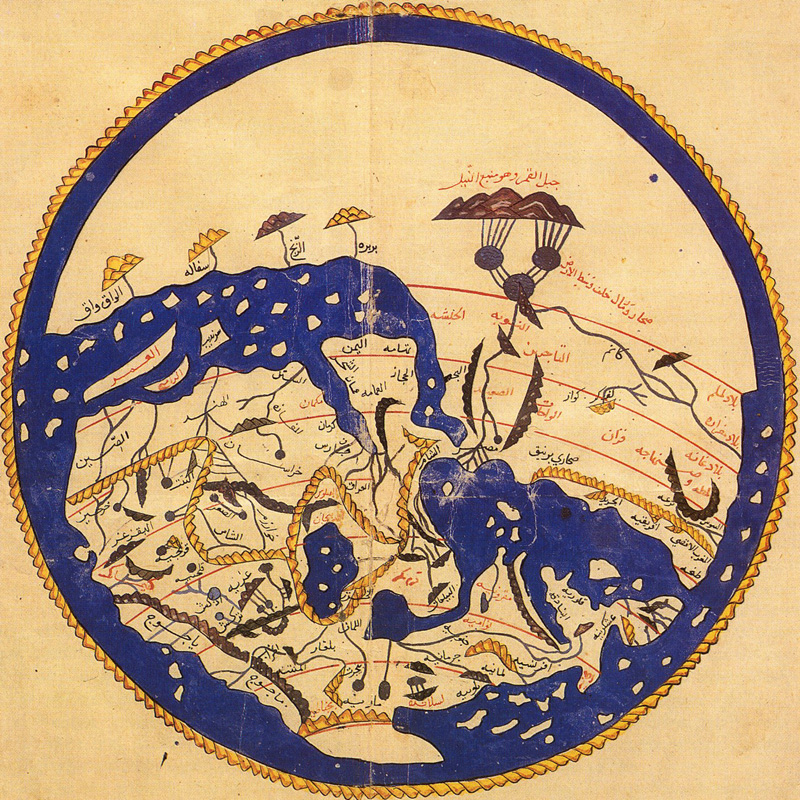
\includegraphics[width=1\textwidth]{figures/1.jpg}}
	\caption{Gambar Peta menurut al-Idrisi}
	\label{Petaal-Idrisi}
	\end{figure}
	\ref{1.jpg} Berikut adalah gambar dari Peta yang dibuat oleh Muhammad al - Idrisi.
	Abu Abdullah Muhammad al-Idrisi al-Qurtubi al-Hasani as-Sabti yang dikenal dengan nama al-Idrisi, hidup antara tahun 1100 – 1165. Al-Idrisi lahir di keluarga Hammudid besar Afrika Utara dan Al-Andalus, yang mengklaim turun dari Idrisids of Morocco dan akhirnya nabi Muhammad. Al-Idrisi lahir di kota Ceuta, di mana kakek buyutnya terpaksa menetap setelah jatuhnya Hammudid Málaga ke Zirids di Granada. Dia menghabiskan sebagian besar masa mudanya untuk bepergian melalui Afrika Utara dan Al-Andalus (Spanyol Muslim saat ini) dan tampaknya telah mendapatkan informasi terperinci mengenai kedua wilayah tersebut. Dia mengunjungi Anatolia saat dia baru berusia 16 tahun. Dia belajar di Córdoba.
	Abu Abdallah Muhammad Al-Idrisi merupakan tokoh saintis islam ynag terkenal pada zamannya.Beliau memberi sumbangan dalam kajian tentang bumi dan alam semesta.Beliau telah mencipta sebuah peta dunia yang pertama di dunia.Beliau telah menerangkan semua tentang permukaan bumi dengan begitu jelas dan teliti.Beliau telah menghasilkan pembagian kaedah dalam kajian permukaan bumi.Pada zaman itu sudah tentu kajian yang dilakukan tanpa menggunakan peralatan atau teknologi yang modern.Beliau menerangkan bahwa bumi ini berbentuk sfera.Antara kaedah yang digunakan seperti penggunaan tali dank au yang berlubang untuk mengira jarak sesuatu tempat dan digunakan sebagai teropong.
	Al-Idrisi berpendapat bahwa pengetahuan tentang Afrika, Samudera Hindia dan Timur Jauh yang digabungkan oleh pedagang dan penjelajah Islam dan dicatat di peta Islam dengan informasi yang dibawa oleh pelayaran Norman untuk membuat peta dunia yang paling akurat pada zaman pra-modern, memiliki tujuan sebagai ilustrasi konkret Kitab nuzhat al-mushtaq-nya, dimana yang bisa dapat diterjemahkan sebagai Pengalihan Manusia untuk Berkelana ke Tempat yang Jauh. 
	Tabula Rogeriana dijelaskan oleh Al-Idrisi di tahun 1154 untuk Raja Norman Roger II dari Sisilia, setelah tinggal delapan belas tahun di istananya, di mana dia mengerjakan komentar dan ilustrasi peta. Peta tersebut, dengan legenda yang ditulis dalam bahasa Arab, sekaligus menunjukkan benua Eurasia secara keseluruhan, hanya menunjukkan bagian utara benua Afrika dan tidak memiliki rincian Tanduk Afrika dan Asia Tenggara.
	\ref{3.jpg} Berikut adalah gambar dari Peta Tabula Rogeriana digambar oleh Al-Idrisi.
	\begin{figure} [ht]
	\centerline{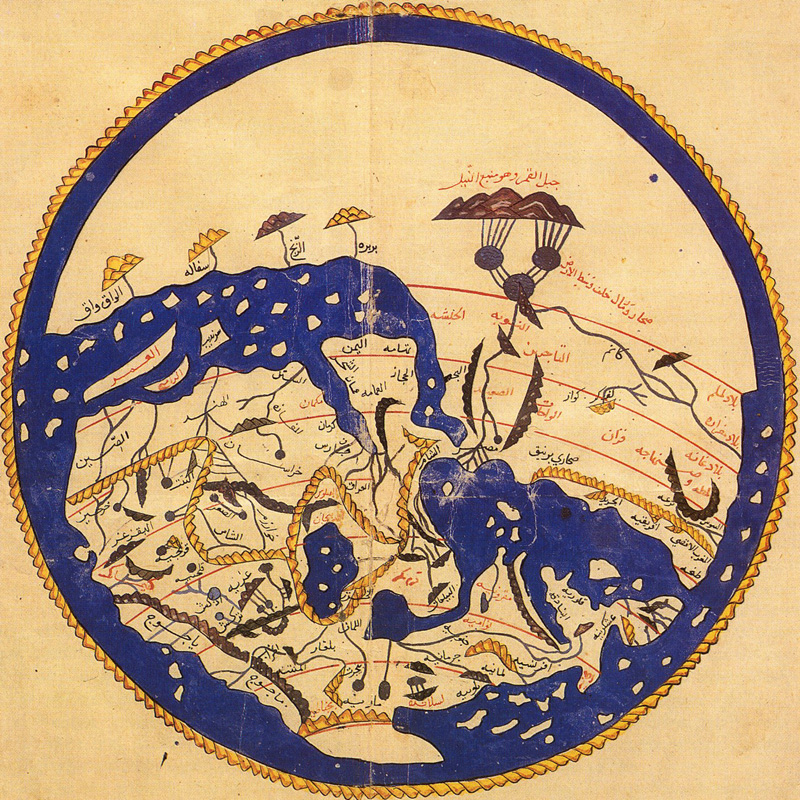
\includegraphics[width=1\textwidth]{figures/1.jpg}}
	\caption{Foto al-Idrisi}
	\end{figure}
	\ref{2.jpg} Foto al-Idrisi seorang ahli geografi,.
	

\subsection {Sejarah Peta dari pandangan Al-Qur'an "al-idrisi"}
	Pandangan Islam mempercayai adanya dua keghaiban, yaitu keghaiban yang eksistensinya tidak harus terukur atau tidak harus difahami melalui metodologi sains, keghaiban yang difahami melalui sistem keimanan, selain itu juga keghaiban yang dikenal sebagai sunattullah. Manusia tak menyaksikan secara langsung tentang proses-proses pembentukan alamsemesta, bahkan kehidupannya di planit Bumi ini hanya merupakan sebagian kecil episode dalam alamsemesta.
	Metodologi sains, Islam memperkenalkan sebuah metodologi lain yaitu ilmupengetahuan (tentang eksistensi kebenaran) bagi manusia bisa bersumber dari sumber terpercaya (kitab Allah) dan disampaikan dengan cara terpercaya. Al Qur’an merupakan sebuah kebenaran yang melengkapi pandangan yang dibangun melalui rasionalitas manusia semata, memperkenalkan Allah sebagai Tuhan alam semesta, ada alam ghaib, ada sesuatu yang ghaib dan manusia tak banyak mengetahuinya, ada cara atau upaya-upaya mencapai atau berkomunikasi dengan Yang MahaPencipta dan MahaPenguasa alam semesta. Pemahaman sunatullah dipergunakan untuk penyempurnaan dan membuat kemudahan-kemudahan dalam hidup dan beribadah agar bisa senantiasa lebih mendekat lagi kepada Allah swt, MahaPencipta dan MahaPenguasa alam semesta.
	Al Qur’an sebagai wahyu Allah yang telah diturunkan kepada umat manusia, perlu dipandang sebagai “resources” bagi kehidupan umat manusia di planit Bumi yaitu sebagai petunjuk Allah swt agar hati manusia bisa tertuntun dan terdidik sehingga berahlak mulia. Gambaran wahyu Allah dalam al Qur'an mengingatkan walaupun ada kepastian dari “tangan-tangan ghaib berupa sunatullah” yang sebagian telah bisa diungkap melalui metodologi sains, namun masih terdapat pengetahuan dan kehendakNya yang ghaib dalam penciptaan Alam Semesta. 
	Pemikiran atas fenomena alam semesta itu sangat diharapkan bisa membangun kesadaran beragama, mempertemukan “kerja tangan-tangan ghaib Allah” yang mengatur alam semesta dengan wahyuNya dalam al Qur’an. Keduanya adalah kebenaran yang berasal dari yang Allah zat yang Maha Esa. Mempertemukan kebenaran wahyu Allah dan ayat kauniyah merupakan proses pemahaman manusia tentang lingkungan kehidupannya yang lebih luas, menjangkau dunia dan akherat, memadukan akal dan keyakinan dalam perspektif Islam. 
	Abad sains dan teknologi telah dijalani manusia, makin tinggi pengetahuan manusia makin diperlukan kesadaran beragama yang lebih tinggi, perlu hidayah yang lebih banyak, agar mendapatkan tuntunanNya sehingga dijauhkan dari bencana sains dan teknologi. 
	Berbagai bentuk upaya-upaya dakwah umat Islam perlu dikembangkan, upaya dakwah hendaknya juga menggerakkan kaum muda masyarakat kampus maupun non kampus dengan wawasan membangun kualitas lingkungan. Agar peran umat Islam dalam hal amar ma’ruf nahi munkar dapat lebih dirasakan dalam masyarakat, perlu dirancang kegiatan yang bersinambung dalam pengembangan, pembelajaran maupun sosialisasi IPTEK. 
	Di abad ke-11 M, seorang geografer termasyhur dari Spanyol, Abu Ubaid Al Bakri berhasil menulis kitab di bidang geografi, yakni Mu’jam Al Ista’jam (Ensiklopedi Geografi) dan Al Masalik wa Al Mamalik (Jalan dan Kerajaan). Buku pertama berisi nama-nama tempat di Jazirah Arab. Sedangkan yang kedua berisi pemetaan geografis dunia Arab zaman dahulu.
	Pada abad ke-12, geografer Muslim Al Idrisi berhasil membuat peta dunia. Al Idrisi yang lahir pada tahun 1100 di Ceuta Spanyol itu juga menulis kitab geografi berjudul Kitab Nazhah Al Muslak fi Ikhtira Al Falak (Tempat Orang yang Rindu Menembus Cakrawala). Kitab ini begitu berpengaruh sehingga diterjemahkan ke dalam bahasa Latin, Geographia Nubiensis.
	Seabad kemudian, dua geografer Muslim yakni Qutubuddin Asy Syirazi (1236 M-1311 M) dan Yaqut Ar Rumi (1179 M-1229 M) berhasil melakukan terobosan baru. Qutubuddin mampu membuat peta Laut Putih atau Laut Tengah yang dihadiahkan kepada Raja Persia. Sedangkan, Yaqut berhasil menulis enam jilid ensiklopedi bertajuk Mu’jam Al Buldan (Ensiklopedi Negeri-negeri).
	Penjelajah Muslim asal Maroko, Ibnu Battutah di abad ke-14 M memberi sumbangan dalam menemukan rute perjalanan baru. Hampir selama 30 tahun, Ibnu Battutah menjelajahi daratan dan mengarungi lautan untuk berkeliling dunia. Penjelajah Muslim lainnya yang mampu mengubah rute perjalanan laut adalah Laksamana Cheng Ho dari Tiongkok. Dia melakukan ekspedisi sebanyak tujuh kali mulai dari tahun 1405 hingga 1433 M.
	Sederet geografer Muslim telah banyak memberi kontribusi bagi pengembangan ilmu bumi. Al Kindi diakui begitu berjasa sebagai geografer pertama yang memperkenalkan percobaan ke dalam ilmu bumi. Sedangkan, Al Biruni didapuk sebagai “bapak geodesi” yang banyak memberi kontribusi terhadap geografi dan juga geologi.
	John J O’Connor dan Edmund F Robertson menuliskan pengakuannya terhadap kontribusi Al Biruni dalam MacTutor History of Mathematics. Menurut mereka, “Al Biruni telah menyumbangkan kontribusi penting bagi pengembangan geografi dan geodesi. Dialah yang memperkenalkan teknik pengukuran bumi dan jaraknya dengan menggunakan triangulation”.
	Al Birunilah yang menemukan radius bumi mencapai 6.339,6 km. Hingga abad ke-16 M, Barat belum mampu mengukur radius bumi seperti yang dilakukan Al Biruni. Bapak sejarah sains, George Sarton juga mengakui kontribusi sarjana Muslim dalam pengembangan geografi dan geologi. “Kita menemukan dalam tulisannya metode penelitian kimia, sebuah teori tentang pembentukan besi”.
	Salah satu kekhasan yang dikembangkan geografer Muslim adalah munculnya bio-geografi. Hal itu didorong oleh banyaknya orang Arab di era kekhalifahan yang tertarik untuk mendistribusi dan mengklasifikasi tanaman, binatang dan evolusi kehidupan. Para sarjana Muslim mencoba menganalisis beragam jenis tanaman.
	Al Idrisi juga seringkali mengkaji berbagai pendapat geografis dari para ahli geografi Arab masa lalu.kegigihan Al Idrisi dalam mengumpulkan dan memahami gambaran berbagai wilayah di muka bumi ini membuatnya dilirik oleh berbagai pihak yang ingin memanfaatkan kecerdasan yang dimilikinya.Diantara penguasa yang mencoba menariknya adalah Roger II,raja Dinasti Normandia dari pulau Sisilia.
	Raja-raja dari Dinasti Normandia banyak menggunakan jasa para ilmuwan Muslim karena dunia Islam pada saat itu saat maju dari segi ilmu pengetahuan.Dibawah pengawasan Roger,Al Idrisi berhasil menuntaskan gambaran dunia secara lengkap seperti yang telah dikenal di dunia Islam pada saat itu.Untuk wilayah-wilayah yang belum dikunjunginyaAl Idrisi mengandalkan data-data dari laporan yang diberikan para pengamat yang dikirimnya ke berbagai tempat dan juga dari informasi yang diberikan oleh orang-orang yang berkunjung ke Sisilia.
	Al Idrisi membuat sebuah peta dunia berukuran bundar yang berwarna keperakan.didalam karya-karyanya ,terdapat banyak hal yang dunia Barat baru mengetahuinya setelah berabad-abad.Contoh Al Idrisi,secara akurat,menunjukkan posisi sumber sungai Nil,yang dianggap Barat sebagai penemuan abad ke-19.Karya-karya Al Idrisi tentang gambaran geografi dunia telah mengubah orang-orang Eropa masa itu yang berpandangan bahwa seluruh dunia,selain Eropa adalah dikuasai oleh orang Muslim.Ini menjadi contoh bagaimana buku geografi dari dunia Islam dapat mempengaruhi dunia keilmuan Barat saat riset atau penelitian geografis yang dilakukan oleh orang Eropa ke daerah Oriental belum dilakukan.
	Sebelum Dinasti Normandia mengambil alih Sisilia,yang berkuasa di daerah itu adalah penguasa Muslim yang telah berkuasa selama berabad-abad.Sehingga,tak mengherankan jika pada saat itu di Sisila terdapat populasi muslim yang cukup banyak.
	Al Idrisi ditempatkan di posisi yang lebih tinggi dari Ibnu Bathutah,karena karyanya yang tidak hanya menitikberatkan pada penjelasan teks seperti dalam karya Ibnu Bathutah,tetapi juga dilengkapi dengan gambaran-gambaran peta yang sangat maju pada zamannya.Al Idrisi,sebgai seorang ahli geografi yang karya-karyanya sangat berpengaruh di zamannya dan setalahnya,sehingga patut disebut didalam daftar yang terdapat pada buku.Semua ini terdapat dalam bukunya yang berjudul Nuzhat Al Mustaq fi Ikhtiraq al Afaq (Rekreasi bagi Orang yan Berhasrat Menjelajahi Berbagai Tempat) atau yan lebih dikenal sebagai Kitab Rujar (Buku Roger).
	\end{flushleft}


